\section{凸性与解的性质}
\label{sec:opt-prob-convexity}

存在性只回答“有没有”。站在一个洼地底部时，我们还想知道：山那边会不会有更深的谷？最低点是不是只有一个？离最低点还有多远？这些问题都涉及两个候选之间的比较，而最简单的比较路径是连接它们的线段。本节先要求线段留在可行域内（凸集），再要求目标沿线段不高于端点的加权平均（凸函数），然后逐步加强这一要求：严格凸排除多个最小点，强凸再给出统一的二次间隔，把目标差换算成到最小点的距离。

\subsection{凸集与凸组合}
\label{sec:opt-prob-convex-sets}

资源分配中，若方案$P=(3,0)$与$Q=(0,4)$都可行，各按一半执行的混合方案$M=\frac12P+\frac12Q=(1.5,2)$也可行：$1.5+2=3.5\leq4$，$3+2=5\leq6$。这不是巧合，因为线性约束在混合下保持：若$\langle\bm g,\bm u\rangle\leq h$且$\langle\bm g,\bm v\rangle\leq h$，则对$\theta\in[0,1]$，$\langle\bm g,\theta\bm u+(1-\theta)\bm v\rangle\leq\theta h+(1-\theta)h=h$。可行方案任意混合仍可行，正是凸集的定义。

\begin{definition}[凸集与凸组合]
\label{def:opt-prob-convex-set}
若对任意$\bm u,\bm v\in C$与$\theta\in[0,1]$都有$\theta\bm u+(1-\theta)\bm v\in C$，称$C\subseteq\mathbb R^d$为\term{凸集}（convex set）。对点$\bm a_1,\dots,\bm a_k$，若$\alpha_i\geq0$且$\sum_{i=1}^k\alpha_i=1$，称$\sum_{i=1}^k\alpha_i\bm a_i$为它们的一个\term{凸组合}（convex combination）。集合$A$中点的全部有限凸组合组成的集合称为$A$的\term{凸包}（convex hull），记作$\operatorname{conv}A$。
\end{definition}

几何上，凸集里任意两点之间的线段都留在集合内。图~\ref{fig:opt-prob-convex-sets}给出对照：椭圆盘中的线段始终在盘内；月牙形中，上下两个尖端附近的点都在集合里，连接它们的线段却穿过缺口；资源分配的四边形里，两个可行方案的混合点$M$落在连接它们的线段上，仍然可行。

\begin{figure}[!htbp]
  \centering
  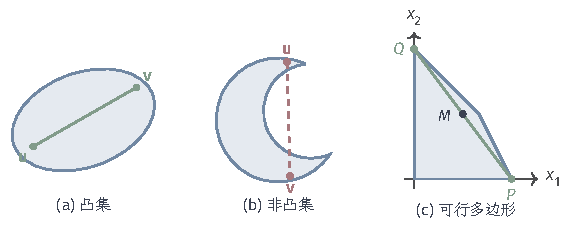
\includegraphics[width=97.017mm]{figures/03-optimization-evolution-and-signals/01-optimization/tikz/c1-convex-sets/figure.pdf}
  \caption{凸集与非凸集。(a) 椭圆盘：任意两点$\bm u,\bm v$之间的线段（绿色）留在集合内。(b) 月牙形：两点都在集合中，连接它们的红色虚线却穿过缺口，所以不是凸集。(c) 资源分配的可行四边形：方案$P=(3,0)$与$Q=(0,4)$的等权混合$M=(1.5,2)$仍在四边形内。}
  \label{fig:opt-prob-convex-sets}
\end{figure}

\paragraph{常见的凸集}
以下几类集合在后文反复出现。对非零$\bm g\in\mathbb R^d$与$h\in\mathbb R$，\term{半空间}（halfspace）$\{\bm x:\langle\bm g,\bm x\rangle\leq h\}$是凸集，上面的计算就是证明。有限个半空间的交称为\term{多面体}（polyhedron），资源分配的可行域$\{\bm x:\bm G\bm x\leq\bm h,\ \bm x\geq\bm 0\}$就是一个多面体，它是第~\ref{chap:opt-linear-programming}章的主角。闭球$\{\bm x:\lVert\bm x-\bm a\rVert_2\leq r\}$是凸集：由三角不等式，$\lVert\theta\bm u+(1-\theta)\bm v-\bm a\rVert_2\leq\theta\lVert\bm u-\bm a\rVert_2+(1-\theta)\lVert\bm v-\bm a\rVert_2\leq r$，对任何范数的球都成立。$d\times d$对称半正定矩阵组成的集合也是凸集：对每个固定的$\bm v$，条件$\bm v^\top\bm X\bm v\geq0$是关于矩阵$\bm X$的线性不等式，半正定矩阵集合是所有这些条件的交。第~\ref{chap:constrained-optimization}章的矩阵约束将用到它。

\paragraph{保持凸性的运算}
判断一个集合是否凸，通常不直接验证定义，而是把它拆成已知凸集经过保凸运算得到的结果。设$\bm M\in\mathbb R^{k\times d}$，$\bm q\in\mathbb R^k$。
\begin{itemize}
  \item 任意多个凸集的交是凸集：两点都在每个集合中，线段也在每个集合中。
  \item 凸集$C\subseteq\mathbb R^d$在仿射映射下的像$\{\bm M\bm x+\bm q:\bm x\in C\}$是凸集：像点的凸组合$\theta(\bm M\bm u+\bm q)+(1-\theta)(\bm M\bm v+\bm q)=\bm M(\theta\bm u+(1-\theta)\bm v)+\bm q$仍是像点。
  \item 凸集$D\subseteq\mathbb R^k$的仿射逆像$\{\bm x:\bm M\bm x+\bm q\in D\}$是凸集：用同一个等式反向读即可。
\end{itemize}
半空间是一维区间$(-\infty,h]$在线性映射$\bm x\mapsto\langle\bm g,\bm x\rangle$下的逆像，多面体是半空间的交，这两条规则就足以确认资源分配可行域是凸集。

\paragraph{凸包与闭凸包}
二点线段可以反复使用。若$C$凸，对点数归纳可知$C$包含其中任意有限个点的凸组合：$k$个点的凸组合在$\alpha_k<1$时可以写成
\[
  \sum_{i=1}^k\alpha_i\bm a_i=(1-\alpha_k)\sum_{i=1}^{k-1}\frac{\alpha_i}{1-\alpha_k}\bm a_i+\alpha_k\bm a_k,
\]
括号里的系数非负且和为$1$，是$k-1$个点的凸组合，再与$\bm a_k$作二点组合；$\alpha_k=1$时组合就是$\bm a_k$本身。另一方面，两个凸组合的凸组合展开后仍是凸组合，所以$\operatorname{conv}A$自身是凸集。二者合起来说明：$\operatorname{conv}A$是包含$A$的最小凸集。资源分配的四边形恰好是它四个顶点的凸包，有界多面体与其顶点的这一关系将在第~\ref{chap:opt-linear-programming}章建立。

凸包不一定是闭集，即使$A$本身闭。取$A=\{(0,0)\}\cup\{(t,1):t\in\mathbb R\}$，它是一个点与一条直线的并，是闭集。原点与直线上的点$(x/y,1)$按权重$1-y$与$y$组合得到$(x,y)$，所以$0<y\leq1$的点都在$\operatorname{conv}A$中；而所有组合的第二个坐标都是权重的平均，非负且只有全部权重给原点时才为零，所以$y=0$的点中只有原点可达。于是$\operatorname{conv}A=\{(0,0)\}\cup\{(x,y):0<y\leq1\}$不闭，它的闭包是带$\{(x,y):0\leq y\leq1\}$。包含$A$的最小闭凸集称为\term{闭凸包}（closed convex hull），它等于$\operatorname{conv}A$的闭包。在需要取极限的论证中，应当用闭凸包而不是凸包；本章只用到这两个对象的定义，一般凸集的分离性质留到后续需要时建立。

\subsection{凸函数与一阶支撑}
\label{sec:opt-prob-convex-functions}

有了凸的可行域，两个可行点之间的线段上都是可行点。接下来要求目标沿这条线段“不鼓起来”：线段上每一点的目标值，不超过两端目标值按相同权重的平均。

\begin{definition}[凸函数]
\label{def:opt-prob-convex-function}
设$C\subseteq\mathbb R^d$为凸集。若函数$f:C\to\mathbb R$对任意$\bm u,\bm v\in C$与$\theta\in[0,1]$满足
\begin{equation}
  f\bigl(\theta\bm u+(1-\theta)\bm v\bigr)\leq\theta f(\bm u)+(1-\theta)f(\bm v),
  \label{eq:opt-prob-convex-function}
\end{equation}
称$f$为$C$上的\term{凸函数}（convex function）。扩展实值函数$f:\mathbb R^d\to\mathbb R\cup\{+\infty\}$称为凸函数，是指$\operatorname{dom}f$为凸集，且式~\eqref{eq:opt-prob-convex-function}对$\operatorname{dom}f$中的点成立。若$-f$凸，称$f$凹。
\end{definition}

式~\eqref{eq:opt-prob-convex-function}的右端是连接$(\bm u,f(\bm u))$与$(\bm v,f(\bm v))$的弦上的点，左端是同一位置的函数值，所以凸函数的图像位于每条弦的下方。图~\ref{fig:opt-prob-chord-tangent}(a)画出了$f(x)=x^2/2$及连接$x=-1$与$x=2$的弦。扩展实值情形只在有效定义域内检验，这避免了$0\cdot(+\infty)$之类无意义的运算；对$F=f_0+\iota_C$，它恰好要求$C$凸且$f_0$在$C$上凸。

\paragraph{上图与Jensen不等式}
另一种看法是把函数图像以上的区域当作一个集合。$f$的\term{上图}（epigraph）是$\operatorname{epi}f=\{(\bm x,s)\in\mathbb R^d\times\mathbb R:\bm x\in\operatorname{dom}f,\ f(\bm x)\leq s\}$。$f$凸当且仅当$\operatorname{epi}f$是凸集。若$f$凸，$(\bm u,s),(\bm v,t)$在上图中，则$f(\theta\bm u+(1-\theta)\bm v)\leq\theta f(\bm u)+(1-\theta)f(\bm v)\leq\theta s+(1-\theta)t$，混合点仍在上图中；反过来，取$s=f(\bm u)$、$t=f(\bm v)$，上图凸就给出式~\eqref{eq:opt-prob-convex-function}。凸函数与凸集因此是同一几何概念的两种说法。

把二点不等式按上一小节的方式对点数归纳，得到有限形式的\term{Jensen不等式}（Jensen's inequality）：对凸函数$f$、$\operatorname{dom}f$中的点$\bm x_1,\dots,\bm x_k$与凸组合系数$\alpha_i$，
\[
  f\Bigl(\sum_{i=1}^k\alpha_i\bm x_i\Bigr)\leq\sum_{i=1}^k\alpha_if(\bm x_i).
\]
系数必须非负且和为$1$：允许负系数时，组合点可以落到这些点的凸包之外，不等式不再有保证。

\paragraph{保凸规则}
与凸集一样，凸函数通常由简单的凸函数拼出来。直接由定义可以验证：凸函数的非负加权和是凸函数；凸函数与仿射映射的复合$\bm x\mapsto f(\bm M\bm x+\bm q)$是凸函数，因为仿射映射把线段映成线段。以最小二乘为例，先验证$\frac12\lVert\cdot\rVert_2^2$凸：展开内积可得恒等式
\begin{equation}
  \theta\lVert\bm u\rVert_2^2+(1-\theta)\lVert\bm v\rVert_2^2-\lVert\theta\bm u+(1-\theta)\bm v\rVert_2^2=\theta(1-\theta)\lVert\bm u-\bm v\rVert_2^2\geq0.
  \label{eq:opt-prob-square-identity}
\end{equation}
于是$\frac12\lVert\bm A\bm x-\bm b\rVert_2^2$是它与仿射映射$\bm x\mapsto\bm A\bm x-\bm b$的复合，$\frac{\lambda}{2}\lVert\bm x\rVert_2^2$是它的非负倍数，二者之和即式~\eqref{eq:opt-prob-ridge}是凸函数。资源分配的目标是线性函数，式~\eqref{eq:opt-prob-convex-function}取等号，既凸又凹。

一般的非线性复合则需要额外条件。$h(u)=u^2$与$k(x)=x^2-1$都是凸函数，复合$h(k(x))=(x^2-1)^2$却不凸：$x=\pm1$处函数值为$0$，中点$x=0$处为$1$，高于弦。一个常用的充分条件是：$k$凸，$h$凸且单调不减。此时$k(\theta u+(1-\theta)v)\leq\theta k(u)+(1-\theta)k(v)$，$h$不减保持这个不等式，再用$h$的凸性即得$h\circ k$凸。上例中$h(u)=u^2$在$u<0$时递减，不满足这一条件。

\paragraph{一阶支撑下界}
凸函数的图像在弦的下方；若函数可微，它还在每一点切线（切平面）的上方。图~\ref{fig:opt-prob-chord-tangent}把两者画在一起：左图凸函数的切线处处位于图像下方，右图非凸函数在$x=0$处的水平切线却位于图像上方的一大段区域。切线来自单点的导数，若它是全局下界，单点信息就能告诉我们远处的函数值至少有多大。这正是凸性在优化中最有用的形式。

\begin{figure}[!htbp]
  \centering
  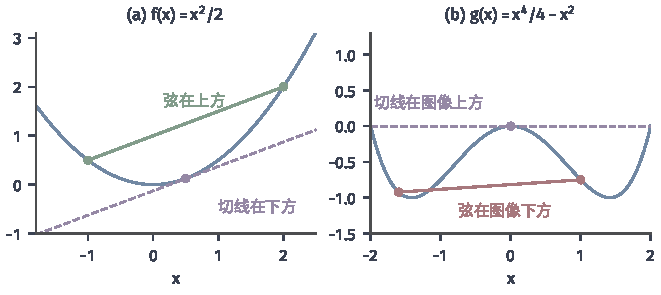
\includegraphics[width=112mm]{figures/03-optimization-evolution-and-signals/01-optimization/matplotlib/c1-chord-tangent/figure.pdf}
  \caption{弦与切线。(a) 凸函数$f(x)=x^2/2$：连接$x=-1$与$x=2$的绿色弦在两点之间位于图像上方，$x_0=1/2$处的紫色切线在整条实轴上位于图像下方。(b) 非凸函数$g(x)=x^4/4-x^2$：连接$x=-1.6$与$x=1$的红色弦有一段位于图像下方，$x=0$处的水平切线在$0<|x|<2$时位于图像上方，不再是下界。}
  \label{fig:opt-prob-chord-tangent}
\end{figure}

\begin{theorem}[凸性的一阶与二阶判据]
\label{thm:opt-prob-convex-criteria}
设$D\subseteq\mathbb R^d$是开凸集，$f:D\to\mathbb R$可微。
\begin{enumerate}
  \item $f$凸，当且仅当对任意$\bm u,\bm v\in D$，
  \begin{equation}
    f(\bm v)\geq f(\bm u)+\langle\nabla f(\bm u),\bm v-\bm u\rangle.
    \label{eq:opt-prob-first-order-support}
  \end{equation}
  \item 若$f$在$D$上二阶可微，则$f$凸当且仅当$\nabla^2f(\bm x)$对每个$\bm x\in D$半正定。
\end{enumerate}
\end{theorem}

\begin{proof}
(1) 设$f$凸。对$t\in(0,1]$，由式~\eqref{eq:opt-prob-convex-function}，$f(\bm u+t(\bm v-\bm u))\leq(1-t)f(\bm u)+tf(\bm v)$，整理得
\[
  \frac{f(\bm u+t(\bm v-\bm u))-f(\bm u)}{t}\leq f(\bm v)-f(\bm u).
\]
令$t\downarrow0$，左端趋于方向导数$\langle\nabla f(\bm u),\bm v-\bm u\rangle$，即得式~\eqref{eq:opt-prob-first-order-support}。反过来，设式~\eqref{eq:opt-prob-first-order-support}对所有点成立。取$\bm z=\theta\bm u+(1-\theta)\bm v$，分别以$\bm z$为切点、$\bm u$与$\bm v$为另一点：
\[
  f(\bm u)\geq f(\bm z)+\langle\nabla f(\bm z),\bm u-\bm z\rangle,\qquad
  f(\bm v)\geq f(\bm z)+\langle\nabla f(\bm z),\bm v-\bm z\rangle.
\]
第一式乘$\theta$、第二式乘$1-\theta$后相加，由$\theta(\bm u-\bm z)+(1-\theta)(\bm v-\bm z)=\bm 0$，内积项抵消，得到式~\eqref{eq:opt-prob-convex-function}。

(2) 设$f$凸，$\bm x\in D$，$\bm h\in\mathbb R^d$。$D$开，$t$充分小时$\bm x+t\bm h\in D$，由式~\eqref{eq:opt-prob-first-order-support}与二阶Taylor展开，
\[
  0\leq f(\bm x+t\bm h)-f(\bm x)-t\langle\nabla f(\bm x),\bm h\rangle=\frac{t^2}{2}\bm h^\top\nabla^2f(\bm x)\bm h+o(t^2).
\]
两端除以$t^2$再令$t\to0$，得$\bm h^\top\nabla^2f(\bm x)\bm h\geq0$。反过来，设Hessian处处半正定。对$\bm u,\bm v\in D$，令$\phi(t)=f(\bm u+t(\bm v-\bm u))$，$t\in[0,1]$，则$\phi''(t)=(\bm v-\bm u)^\top\nabla^2f(\bm u+t(\bm v-\bm u))(\bm v-\bm u)\geq0$，$\phi'$单调不减。一元函数导数单调不减时函数凸（由中值定理可得），所以$\phi(\theta\cdot0+(1-\theta)\cdot1)\leq\theta\phi(0)+(1-\theta)\phi(1)$，这正是式~\eqref{eq:opt-prob-convex-function}。
\end{proof}

定理中的Taylor展开与Hessian的计算见卷一；这里要强调的是两个判据的适用范围。它们都要求在整个开凸集上成立：在单个点检查Hessian半正定，不能证明函数凸。示例~\ref{ex:opt-prob-local-global}中的$f(x)=x^4/4-x^3/3-x^2$满足$f''(2)=6>0$，但$f''(0)=-2<0$，所以$f$不凸，也正因为不凸，它才会有不是全局最优的局部最优。对最小二乘，$\nabla^2f=\bm A^\top\bm A+\lambda\bm I$，对任意$\bm h$有$\bm h^\top(\bm A^\top\bm A+\lambda\bm I)\bm h=\lVert\bm A\bm h\rVert_2^2+\lambda\lVert\bm h\rVert_2^2\geq0$，与前面用保凸规则得到的结论一致。

\paragraph{局部最优即全局最优}
现在可以回答“山那边会不会有更深的谷”。

\begin{theorem}[凸问题的局部最优是全局最优]
\label{thm:opt-prob-local-global}
设$C$为凸集，$f:C\to\mathbb R$为凸函数。则$f$在$C$上的每个局部最优解都是全局最优解，并且最优解集合是凸集。
\end{theorem}

\begin{proof}
设$\bm u$是局部最优解，邻域半径为$r$。若存在$\bm v\in C$使$f(\bm v)<f(\bm u)$，对$t\in(0,1)$，点$\bm u+t(\bm v-\bm u)$在$C$中，且
\[
  f(\bm u+t(\bm v-\bm u))\leq(1-t)f(\bm u)+tf(\bm v)<f(\bm u).
\]
取$t$足够小，使$t\lVert\bm v-\bm u\rVert_2<r$，这个更低的点落在$C\cap B(\bm u,r)$中，与局部最优矛盾。所以$\bm u$是全局最优解。若$\bm u,\bm v$都是最优解，线段上的点满足$f\leq\theta f^\star+(1-\theta)f^\star=f^\star$，也是最优解，故最优解集合凸。
\end{proof}

证明的几何意义是：如果远处有更低的点，连向它的线段会从当前点出发立即下降，“假谷底”不可能存在。证明没有用到可微性，对非光滑的凸目标同样成立。最小二乘实例在$\lambda=0$时的最优解集合是一条直线，与定理的“最优解集合凸”一致。凸集与凸函数的系统处理可参考Boyd与Vandenberghe的教材\scite{math-boyd2004convex}。

\subsection{严格凸性与唯一性}
\label{sec:opt-prob-strict-convexity}

凸性排除了“假谷底”，但没有排除平坦的谷底：$\lambda=0$的最小二乘实例沿直线$x_1+x_2=2$处处最优。要让最优解唯一，需要线段上的不等式在两端不同时严格成立。

\begin{definition}[严格凸函数]
\label{def:opt-prob-strict-convex}
设$C$为凸集，$f:C\to\mathbb R$。若对任意$\bm u\neq\bm v$与$\theta\in(0,1)$，式~\eqref{eq:opt-prob-convex-function}严格成立，称$f$为\term{严格凸}（strictly convex）函数。
\end{definition}

\begin{theorem}[严格凸目标至多有一个最小点]
\label{thm:opt-prob-strict-unique}
设$C$为凸集，$f$在$C$上严格凸，则$\argmin_{\bm x\in C}f$至多含一个点。若再有最优解存在，则最优解唯一。
\end{theorem}

\begin{proof}
若$\bm u\neq\bm v$都是最优解，则中点$\frac12(\bm u+\bm v)\in C$满足$f(\frac12(\bm u+\bm v))<\frac12f^\star+\frac12f^\star=f^\star$，与$f^\star$是下确界矛盾。
\end{proof}

定理的结论是“至多一个”，存在性必须另外由上一节的条件保证。正反两个方向都有反例。$e^x$在$\mathbb R$上严格凸（二阶导数处处为正），却没有最小点：严格凸不推出存在。$|x|$有唯一最小点$0$，但在$[0,1]$上是线性的，式~\eqref{eq:opt-prob-convex-function}取等号，不严格凸：最小点唯一不推出严格凸。资源分配是一个更实际的例子：线性目标处处不严格凸，最优解$(2,2)$却是唯一的，唯一性来自可行域的顶点，而不是目标的弯曲。

\paragraph{二次函数的一个恒等式}
最小二乘是二次函数，严格凸可以直接读出来。设$q(\bm x)=\frac12\bm x^\top\bm H\bm x+\bm g^\top\bm x+c$，$\bm H$对称。仿照式~\eqref{eq:opt-prob-square-identity}展开，线性项与常数项在加权平均中抵消，得到
\begin{equation}
  \theta q(\bm u)+(1-\theta)q(\bm v)-q\bigl(\theta\bm u+(1-\theta)\bm v\bigr)=\frac12\theta(1-\theta)(\bm u-\bm v)^\top\bm H(\bm u-\bm v).
  \label{eq:opt-prob-quadratic-identity}
\end{equation}
左端是弦与函数之间的间隔，它完全由$\bm H$在方向$\bm u-\bm v$上的二次型决定。于是$q$凸当且仅当$\bm H$半正定，严格凸当且仅当$\bm H$正定：若$\bm H$半正定但奇异，取零空间中的非零方向$\bm w$，沿该方向的线段上间隔为零，不严格凸。

最小二乘目标展开为$f(\bm x)=\frac12\bm x^\top(\bm A^\top\bm A+\lambda\bm I)\bm x-\bm b^\top\bm A\bm x+\frac12\lVert\bm b\rVert_2^2$，$\bm H=\bm A^\top\bm A+\lambda\bm I$。对非零$\bm w$，$\bm w^\top\bm H\bm w=\lVert\bm A\bm w\rVert_2^2+\lambda\lVert\bm w\rVert_2^2$。$\lambda>0$时它为正；$\lambda=0$时它为正当且仅当$\bm A\bm w\neq\bm 0$对所有非零$\bm w$成立，即$\bm A$列满秩。所以$\lambda>0$或$\bm A$列满秩时目标严格凸，再结合上一节的存在性，最优解唯一。在最小二乘实例中，$\bm H=\begin{pmatrix}1+\lambda&1\\1&1+\lambda\end{pmatrix}$；$\lambda=0$时$\bm w=(1,-1)$使$\bm w^\top\bm H\bm w=0$，最优解成线；$\lambda>0$时最优条件$(\bm A^\top\bm A+\lambda\bm I)\bm x=\bm A^\top\bm b=(2,2)^\top$有唯一解$\bm x^\star=\frac{2}{2+\lambda}(1,1)$，$\lambda=0.5$时即图~\ref{fig:opt-prob-ls-sublevel}(b)中的$(0.8,0.8)$。

\subsection{强凸性与误差控制}
\label{sec:opt-prob-strong-convexity}

严格凸只说弦与函数之间有间隔，没说间隔有多大。$x^4$严格凸，但在原点附近极其平坦：取$\bm u=-t$、$\bm v=t$、$\theta=\frac12$，间隔只有$\frac12t^4+\frac12t^4-0=t^4$，比两点距离的平方$4t^2$小得多。若间隔太小，目标值几乎相同的两个点可能相距很远，我们就无法从“目标值差不多最优”推断“参数差不多正确”。强凸性要求间隔至少与距离的平方成比例。

\begin{definition}[强凸性]
\label{def:opt-prob-strong-convex}
设$C$为凸集，$f:C\to\mathbb R$，$\lVert\cdot\rVert$是$\mathbb R^d$上的一个范数，$\mu>0$。若对任意$\bm u,\bm v\in C$与$\theta\in[0,1]$，
\begin{equation}
  f\bigl(\theta\bm u+(1-\theta)\bm v\bigr)\leq\theta f(\bm u)+(1-\theta)f(\bm v)-\frac{\mu}{2}\theta(1-\theta)\lVert\bm u-\bm v\rVert^2,
  \label{eq:opt-prob-strong-convexity}
\end{equation}
称$f$在$C$上关于$\lVert\cdot\rVert$是\term{$\mu$强凸}（$\mu$-strongly convex）的。未注明范数时指欧氏范数$\lVert\cdot\rVert_2$。
\end{definition}

与式~\eqref{eq:opt-prob-quadratic-identity}比较，强凸性要求每条弦下方至少留出一个“抛物线形”的间隔$\frac{\mu}{2}\theta(1-\theta)\lVert\bm u-\bm v\rVert^2$。对二次函数$q$，由式~\eqref{eq:opt-prob-quadratic-identity}，它关于$\lVert\cdot\rVert_2$是$\mu$强凸的当且仅当$\bm w^\top\bm H\bm w\geq\mu\lVert\bm w\rVert_2^2$对所有$\bm w$成立。对称矩阵二次型与特征值的关系给出$\bm w^\top\bm H\bm w\geq\lambda_{\min}(\bm H)\lVert\bm w\rVert_2^2$，取$\bm w$为最小特征值的特征向量时取等号（可参考\BookChapterRef{chap:linear-analysis}{卷一“谱和奇异值”章}），所以最大的强凸常数是$\mu=\lambda_{\min}(\bm H)$。对最小二乘，$\lambda_{\min}(\bm A^\top\bm A+\lambda\bm I)=\lambda_{\min}(\bm A^\top\bm A)+\lambda\geq\lambda$。实例中$\bm H$的特征值为$\lambda$（特征向量$(1,-1)$）与$2+\lambda$（特征向量$(1,1)$），所以$\mu=\lambda$：正则系数恰好就是强凸常数。

\paragraph{欧氏情形的等价形式}
在欧氏范数下，强凸性可以化归为普通凸性。由式~\eqref{eq:opt-prob-square-identity}，$\frac{\mu}{2}\lVert\cdot\rVert_2^2$的弦间隔恰好是$\frac{\mu}{2}\theta(1-\theta)\lVert\bm u-\bm v\rVert_2^2$，所以式~\eqref{eq:opt-prob-strong-convexity}等价于：$g=f-\frac{\mu}{2}\lVert\cdot\rVert_2^2$是凸函数。把定理~\ref{thm:opt-prob-convex-criteria}用于$g$，在开凸集上可微时，$f$为$\mu$强凸等价于
\begin{equation}
  f(\bm v)\geq f(\bm u)+\langle\nabla f(\bm u),\bm v-\bm u\rangle+\frac{\mu}{2}\lVert\bm v-\bm u\rVert_2^2,
  \label{eq:opt-prob-strong-first-order}
\end{equation}
即函数位于每点切平面加上一个开口为$\mu$的抛物面之上；二阶可微时又等价于$\nabla^2f(\bm x)-\mu\bm I$处处半正定。这个化归也给出不可微的例子：$f(x)=x^2/2+|x-0.5|$等于$\frac12x^2$加上凸函数$|x-0.5|$，所以是$1$强凸的，尽管在$x=0.5$处不可微。图~\ref{fig:opt-prob-strong-convex-gap}(a)画出了它的弦与“弦减去二次间隔”：函数图像始终在虚线下方。对一般范数，$\lVert\cdot\rVert^2$未必是二次型，Hessian形式不再适用，应回到定义~\ref{def:opt-prob-strong-convex}。

\begin{figure*}[!htbp]
  \centering
  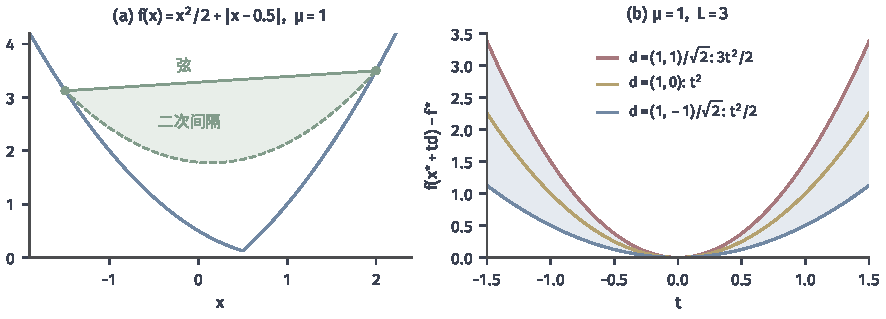
\includegraphics[width=150mm]{figures/03-optimization-evolution-and-signals/01-optimization/matplotlib/c1-strong-convex-gap/figure.pdf}
  \caption{强凸性的二次间隔。(a) $f(x)=x^2/2+|x-0.5|$是$1$强凸的：连接$u=-1.5$与$v=2$的绿色弦下方，虚线是弦减去$\frac{1}{2}\theta(1-\theta)(u-v)^2$，函数图像（蓝）始终不高于虚线，浅绿区域是强凸性保证的间隔。(b) 最小二乘实例取$\lambda=1$，$\bm H=\begin{pmatrix}2&1\\1&2\end{pmatrix}$，特征值为$1$与$3$；沿三个单位方向$\bm d$画出$f(\bm x^\star+t\bm d)-f^\star=\frac12t^2\bm d^\top\bm H\bm d$，所有曲线都夹在$\frac12t^2$与$\frac32t^2$之间（浅蓝带）。}
  \label{fig:opt-prob-strong-convex-gap}
\end{figure*}

\paragraph{目标差控制到最小点的距离}
强凸性最直接的用途，是把目标值的误差换成参数的误差。

\begin{theorem}[强凸目标的二次增长]
\label{thm:opt-prob-strong-growth}
设$C$为凸集，$f$在$C$上关于范数$\lVert\cdot\rVert$为$\mu$强凸，且$\bm x^\star\in\argmin_{\bm x\in C}f$存在。则对所有$\bm x\in C$，
\begin{equation}
  f(\bm x)-f^\star\geq\frac{\mu}{2}\lVert\bm x-\bm x^\star\rVert^2,
  \qquad\text{从而}\qquad
  \lVert\bm x-\bm x^\star\rVert\leq\sqrt{\frac{2\bigl(f(\bm x)-f^\star\bigr)}{\mu}}.
  \label{eq:opt-prob-quadratic-growth}
\end{equation}
特别地，最优解唯一。
\end{theorem}

\begin{proof}
对$t\in(0,1)$，点$\bm x^\star+t(\bm x-\bm x^\star)$在$C$中，其目标值不低于$f^\star$。在式~\eqref{eq:opt-prob-strong-convexity}中取$\bm u=\bm x$、$\bm v=\bm x^\star$、$\theta=t$：
\[
  f^\star\leq f\bigl(\bm x^\star+t(\bm x-\bm x^\star)\bigr)\leq tf(\bm x)+(1-t)f^\star-\frac{\mu}{2}t(1-t)\lVert\bm x-\bm x^\star\rVert^2.
\]
整理并除以$t>0$，得$f(\bm x)-f^\star\geq\frac{\mu}{2}(1-t)\lVert\bm x-\bm x^\star\rVert^2$；令$t\downarrow0$即得式~\eqref{eq:opt-prob-quadratic-growth}。若$\bm x$也是最优解，左端为零，迫使$\bm x=\bm x^\star$。
\end{proof}

证明只用到可行域凸、目标强凸和最小点存在，没有假设最小点在内部或目标可微，所以对约束问题与非光滑目标同样成立。以实例$\lambda=1$为例，$\bm x^\star=(2/3,2/3)$，$\mu=1$。取$\bm x=\bm x^\star+(1,-1)=(5/3,-1/3)$，由于最优点处梯度为零，二次函数的展开给出$f(\bm x)-f^\star=\frac12(1,-1)\bm H(1,-1)^\top=1$；式~\eqref{eq:opt-prob-quadratic-growth}给出距离上界$\sqrt{2\cdot1/1}=\sqrt2$，恰好等于实际距离，因为位移方向正是最小特征值的特征向量。

\paragraph{曲率下界与曲率上界}
图~\ref{fig:opt-prob-strong-convex-gap}(b)展示了同一个二次函数沿不同方向离开最小点时的增长。无约束且$\nabla f(\bm x^\star)=\bm 0$时，$f(\bm x)-f^\star=\frac12(\bm x-\bm x^\star)^\top\bm H(\bm x-\bm x^\star)$，因此
\[
  \frac{\lambda_{\min}(\bm H)}{2}\lVert\bm x-\bm x^\star\rVert_2^2\leq f(\bm x)-f^\star\leq\frac{\lambda_{\max}(\bm H)}{2}\lVert\bm x-\bm x^\star\rVert_2^2.
\]
下界来自强凸常数$\mu$，它说明目标差小时参数不可能离得太远；上界来自曲率的上限，它说明参数接近时目标差也小。对一般函数，上界对应梯度的Lipschitz常数$L$，第~\ref{chap:opt-smooth}章将系统使用$L$与$\mu$及其比值$\kappa=L/\mu$。两个常数回答的是相反方向的问题，不能互相替代。

\paragraph{可行域必须凸}
定理~\ref{thm:opt-prob-strong-growth}要求可行域凸，这一条件不能省略。$f(x)=x^2$在$\mathbb R$上$2$强凸，但在非凸集$C=\{x:|x|\geq1\}$上有两个最小点$\pm1$。取$\bm x^\star=-1$与$x=1$，目标差为$0$，距离却是$2$，式~\eqref{eq:opt-prob-quadratic-growth}不成立：证明中从$\bm x^\star$走向$\bm x$的线段离开了可行域。后续各章只在确有凸可行域与相应常数时才使用这类误差换算。
